\documentclass{report}
\usepackage[utf8]{inputenc}
\usepackage[T1]{fontenc}
\usepackage[brazil]{babel}
\usepackage{graphicx}
\usepackage{amsfonts}
\usepackage{amssymb}
\usepackage{amsmath}
\usepackage{multicol}
\usepackage{ifthen}
\newboolean{firstanswerofthechapter}  
\usepackage{xcolor}
\colorlet{lightcyan}{cyan!40!white}
\usepackage{chngcntr}
\usepackage{stackengine}
\usepackage{tasks}
\usepackage{multirow}
\usepackage{float}
\newlength{\longestlabel}
\settowidth{\longestlabel}{\bfseries viii.}
%\settasks{counter-format={tsk[r].}, label-format={\bfseries}, label-width=\longestlabel,
    %item-indent=0pt, label-offset=2pt, column-sep={10pt}}
		
% \setcounter{secnumdepth}{0} \setlength{\topmargin}{0cm}
% \setlength{\headsep}{-2cm} \setlength{\textwidth}{17.5cm}
% \setlength{\textheight}{23cm} \setlength{\oddsidemargin}{-0.8cm}
% \setlength{\evensidemargin}{0cm} \setlength{\footskip}{-1.5cm}

\usepackage[left=1.5cm,right=1.5cm,top=2cm,bottom=0.5cm,includefoot]{geometry}
		
\usepackage[lastexercise,answerdelayed]{exercise}
%\counterwithin{Exercise}{chapter}
%\counterwithin{Answer}{chapter}
%\renewcounter{Exercise}[chapter]
%\newcommand{\QuestionNB}{\bfseries\arabic{Question}.\ }
%\renewcommand{\ExerciseName}{Exercício}
%\renewcommand{\ExerciseHeader}{\noindent\def\stackalignment{l}% code from https://tex.stackexchange.com/a/195118/101651
    %\stackunder[0pt]{\colorbox{cyan}{\textcolor{white}{\textbf{\LARGE\ExerciseHeaderNB\;\large\ExerciseName}}}}{\textcolor{lightcyan}{\rule{\linewidth}{2pt}}}\medskip}
\renewcommand{\ExerciseName}{Exercícios}
\renewcommand{\ExerciseHeader}{\noindent\def\stackalignment{l}% code from https://tex.stackexchange.com/a/195118/101651
    \stackunder[0pt]{\colorbox{gray}{\textcolor{white}{\textbf{\large\ExerciseName}}}}{\textcolor{lightgray}{\rule{\linewidth}{2pt}}}\medskip}
%\renewcommand{\AnswerName}{Exercises}
%\renewcommand{\AnswerHeader}{\ifthenelse{\boolean{firstanswerofthechapter}}%
    %{\bigskip\noindent\textcolor{cyan}{\textbf{CHAPTER \thechapter}}\newline\newline%
        %\noindent\bfseries\emph{\textcolor{cyan}{\AnswerName\ \ExerciseHeaderNB, page %
                %\pageref{\AnswerRef}}}\smallskip}
    %{\noindent\bfseries\emph{\textcolor{cyan}{\AnswerName\ \ExerciseHeaderNB, page \pageref{\AnswerRef}}}\smallskip}}
%\setlength{\QuestionIndent}{16pt}

\usepackage{Sweave}
\begin{document}
\Sconcordance{concordance:Lista1.tex:Lista1.Rnw:%
1 52 1 1 0 346 1}



\vspace*{-2cm}

\begin{center}
\begin{minipage}[s]{4cm}
\hspace{-1.3cm}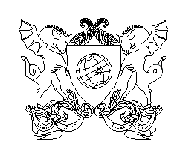
\includegraphics[scale=1.0]{Figuras/brasaoufv.eps}
\end{minipage}
\begin{minipage}[s]{13cm}
{\begin{center} {\sc \Large Universidade Federal de Vi\c{c}osa}\\
{\sc \large Instituto de Ci\^encias Exatas e Tecnológicas}\\
{\sc \large Campus UFV - Florestal}\\
\end{center}}
\end{minipage}\begin{minipage}[s]{2 cm}
%\includegraphics[width=2 cm]{logoimecc.eps}
\end{minipage}
\end{center}

\vspace{-0.3cm}

%\hline \hline \noindent

%%%%%%%%%%%%%%%%%%%%%%%%%%%%%%%%%%%%%%%%%%%%%%%%%%%%%%%%%%%%%%%%%%%%%%%%%%%

\medskip

\begin{center}

\underline{\underline{{\large{\sc Lista de Iniciação Estatística - Lista 1}}}}

\bigskip

{\large {\bf Prof. Fernando Bastos}}
%\bigskip
%
\end{center}

\begin{Exercise}

\Question Represente as somas utilizando somatórios:
\begin{tasks}(2)
\task $x_{1}y_{1}+x_{2}y_{2}+\cdots x_{10}y_{10};$
\task $1+2+3+4+5+\cdots$
\task $1+2^{3}+3^{4}+4^{5}+\cdots+100^{101};$
\task $1+2^{2}+3^{3}+\cdots+30^{30};$
\task $\dfrac{1}{z_{1}}+\dfrac{2}{z_{2}}+\cdots+\dfrac{r}{z_{r}};$
\task $\dfrac{1}{2}+\dfrac{2}{3}+\cdots+\dfrac{n}{n+1};$
\task $(a_{2}-b_{1})+(a_{3}-b_{2})+\cdots+(a_{50}-b_{49});$
\task $a_{0}+a_{1}x+a_{2}x^{2}+\cdots+a_{10x^{10}};$
\end{tasks} 
$\newline$
\Question Desenvolva cada uma das somas indicadas:
\begin{tasks}(2)
\task ${\displaystyle \sum_{j=1}^{6}x_{j}};$
\task ${\displaystyle \sum_{i=1}^{6}(x_{i}-k)};$
\task ${\displaystyle \sum_{i=2}^{10}k};$
\task ${\displaystyle \sum_{j=1}^{10}z_{j}(z_{j}+2)};$
\task ${\displaystyle \sum_{i=1}^{4}x_{i}^{2}};$
\task ${\displaystyle \sum_{i=1}^{5}x_{i}^{2-i}};$
\task ${\displaystyle \sum_{j=1}^{6}5j};$
\task ${\displaystyle \sum_{i=-2}^{2}i^{3}};$
\end{tasks} 
$\newline$
\Question Verdadeiro ou Falso:
\begin{tasks}(2)
\task (\ ) ${\displaystyle \sum_{i=0}^{200}i^{3}=\sum_{i=1}^{200}i^{3}};$
\task (\ ) ${\displaystyle \sum_{i=0}^{n}i=\dfrac{n(n+1)}{2}};$
\task (\ ) ${\displaystyle \sum_{i=0}^{n}i^{2}=\dfrac{n(n+1)(2n+1)}{6}};$
\task (\ ) ${\displaystyle \sum_{s=0}^{1000}(3+s)=3+\sum_{s=0}^{1000}s};$
\task (\ ) ${\displaystyle \sum_{k=1}^{n}2k=2\sum_{k=1}^{n}k};$
\task (\ ) ${\displaystyle \sum_{i=0}^{n}i^{2}=\Biggl(\sum_{i=0}^{n}i\Biggl)^{2}};$
\task (\ ) ${\displaystyle \sum_{l=8}^{32}(3+l)=75+\sum_{l=8}^{32}l};$
\task (\ ) ${\displaystyle \sum_{i=5}^{200}(a_{i}+b_{i})=\sum_{i=5}^{m}a_{i}+\sum_{i=5}^{m}b_{i}};$
\end{tasks}

\newpage

\Question Sabendo-se que ${\displaystyle \sum_{i=1}^{10}X_{i}=-6}$ e que 
${\displaystyle \sum_{i=1}^{10}X_{i}^{2}=12},$ calcule:

\begin{tasks}(2)
\task  ${\displaystyle \dfrac{\displaystyle\sum_{i=1}^{10}X_{i}^{2}-\dfrac{\left(\displaystyle\sum_{i=1}^{10}X_{i}\right)^{2}}{10}}{10-1}}$
\task  ${\displaystyle \sum_{i=1}^{10}X_{i}(X_{i}-2)}$
\task  ${\displaystyle \sum_{i=1}^{10}(X_{i}-3)^{2}}$
\task  ${\displaystyle \sum_{i=1}^{10}(4X_{i}+5)}$
\task  ${\displaystyle \sum_{i=1}^{10}(X_{i}-4)}$
\task  ${\displaystyle \sum_{i=1}^{10}(X_{i}-4)^{2}}$
\task  ${\displaystyle \dfrac{ \sum_{i=1}^{10}(X_{i}-4)^{2}}{10-1}}$
\task  ${\displaystyle \dfrac{\sum_{i=1}^{10}X_{i}}{10}}$
\end{tasks}
$\newline$
\Question Utilizando os dados da tabela abaixo, referente aos valores $X_{ij}$ calcule o resultado numérico quando possível:

$$
\begin{tabular}{c|cccc}
  \hline
  % after \\: \hline or \cline{col1-col2} \cline{col3-col4} ...
  i$\setminus$ j & 1 & 2 & 3 & 4 \\
  \hline
  1 & 8 & 7 & 5 & 9 \\
  2 & 4 & 0 & 10 & 2 \\
  \hline
\end{tabular}
$$

\begin{tasks}(2)
\task  ${\displaystyle \sum_{i=1}^{2}X_{i1}}$
\task  ${\displaystyle \sum_{j=1}^{4}X_{1j}}$
\task  ${\displaystyle \sum_{j=1 \atop j\neq 3}^{4}X_{ij}}$
\task  ${\displaystyle \sum_{j=2}^{3}X_{2j}}$
\task  ${\displaystyle \sum_{j=1 \atop j\neq 2}^{4}\dfrac{1}{X_{2j}}}$
\task  ${\displaystyle \prod_{j=1 \atop j\neq 3}^{4}6X_{1j}}$
\task  ${\displaystyle \prod_{j=1 \atop j\neq 2}^{4}X_{2j}}$
\end{tasks}
$\newline$
\Question Escrever usando notação de somatório ou produtório, conforme o caso:

\begin{tasks}(2)
\task ${\displaystyle \left(\dfrac{X_{1}-Y_{1}}{2}+\dfrac{X_{2}-Y_{2}}{2}+\dfrac{X_{4}-Y_{4}}{2}\right)^{2}}$
\task ${\displaystyle a!}$
\task ${\displaystyle (X_{1}+Y_{1})(X_{1}+Y_{2})(X_{1}+Y_{3})}$
\task ${\displaystyle (X_{1}Y_{1})+(X_{1}Y_{2})+(X_{1}Y_{3})+(X_{2}Y_{1})+(X_{2}Y_{2})+(X_{2}Y_{3})}$
\task ${\displaystyle (X_{1}Y_{1}).(X_{2}Y_{2}).\ldots.(X_{n}Y_{n})}$
\task ${\displaystyle x_{1}^{2}+x_{2}^{2} \cdots x_{n}^{2}}$
\task ${\displaystyle [(b_{1}-2):(w_{1}+4)]^{8}+\cdots+[(b_{20}-2):(w_{20}+4)]^{8}}$
\task ${\displaystyle a_{1}b_{1}+a_{3}b_{3}+\cdots+a_{25}b_{25}}$
\task ${\displaystyle \log{x_{1}}+\log{x_{2}}+\cdots+\log{x_{n}}}$
\task ${\displaystyle (kx_{1})(kx_{2})(kx_{3})\cdots(kx_{n})}$
\end{tasks}
$\newline$
\Question Se $X_{1}=2,\quad X_{2}=4,\quad X_{3}=6$\quad e\quad $Y_{1}=3,\quad Y_{2}=5,\quad Y_{3}=6,$ calcule:


\begin{tasks}(2)
\task ${\displaystyle \sum_{i=1}^{3}\left(X_{i}Y_{i}\right)}$
\task ${\displaystyle \sum_{i=1}^{3}\left(X_{i}-2\right)\left(Y_{i}-5\right)}$
\end{tasks}

\end{Exercise}

\end{document}
